% =============================================================================
%  PageIndex on CLEVRER: pilot results (research meeting, 12 Oct 2026)
%  Build: latexmk -pdf -outdir=tmp pilot-results.tex   (figures come from ../results/)
% =============================================================================
\documentclass[aspectratio=169,11pt]{beamer}

\usepackage[T1]{fontenc}
\usepackage[utf8]{inputenc}
\usepackage[sfdefault]{plex-sans}
\usepackage{plex-mono}
\usepackage{microtype}
\usepackage[document]{ragged2e}
\usepackage{booktabs}
\usepackage{array}
\usepackage{graphicx}
\usepackage{tikz}
\usepackage{hyperref}
\graphicspath{{../results/}}

\hyphenpenalty=10000
\exhyphenpenalty=10000
\tolerance=3000

% ---------------------------------------------------------------------- palette
\definecolor{Ink}{HTML}{1A1C1E}
\definecolor{Body}{HTML}{303338}
\definecolor{Mute}{HTML}{74787E}
\definecolor{Rule}{HTML}{D3D6D9}
\definecolor{Panel}{HTML}{F2F3F4}
\definecolor{Accent}{HTML}{23405E}
\definecolor{Neg}{HTML}{8A3A2C}
\definecolor{PIblue}{HTML}{2A78D6}
\definecolor{FCorange}{HTML}{EB6834}
\definecolor{GAaqua}{HTML}{1BAF7A}

\setbeamercolor{background canvas}{bg=white}
\setbeamercolor{normal text}{fg=Body}
\setbeamercolor{frametitle}{fg=Ink}
\setbeamercolor{structure}{fg=Accent}
\setbeamerfont{normal text}{size=\fontsize{12}{15.5}}
\setbeamersize{text margin left=1.15cm,text margin right=1.15cm}

\setbeamertemplate{navigation symbols}{}
\setbeamertemplate{itemize item}{\color{Mute}\raise0.25ex\hbox{\rule{0.45ex}{0.45ex}}}
\setbeamertemplate{itemize subitem}{\color{Mute}\raise0.25ex\hbox{\rule{0.35ex}{0.35ex}}}

\setbeamerfont{frametitle}{series=\bfseries,size=\fontsize{16.5}{20}}
\setbeamertemplate{frametitle}{%
  \vspace{0.30cm}%
  \insertframetitle\par%
  \vspace{0.11cm}%
  {\color{Rule}\rule{\textwidth}{0.5pt}}%
}

\setbeamerfont{footline}{size=\fontsize{7.5}{9}}
\setbeamertemplate{footline}{%
  \leavevmode%
  \hbox{%
    \begin{beamercolorbox}[wd=\paperwidth,ht=0.26cm,dp=0.20cm,%
                           rightskip=1.15cm plus1fil]{footline}%
      \color{Mute}\hfill\insertframenumber
    \end{beamercolorbox}%
  }%
}

% ---------------------------------------------------------------------- helpers
\newcommand{\lbl}[1]{{\color{Mute}\fontsize{9.5}{12}\selectfont #1}\par}
\newcommand{\finding}[2]{%
  \noindent{\color{Accent}\fontsize{16}{19}\selectfont\bfseries #1}%
  \hspace{0.28em}{\color{Body}\fontsize{10.5}{13.5}\selectfont #2}\par}
\newcommand{\fnote}[1]{{\color{Mute}\fontsize{8.5}{11}\selectfont #1\par}}
\newcommand{\code}[1]{{\ttfamily\fontsize{8.6}{11.4}\selectfont #1}}
\newcommand{\sw}[1]{\tikz[baseline=-0.6ex]\fill[#1] (0,-0.09) rectangle (0.22,0.13);}

\begin{document}

% == 1 == Title ================================================================
\begin{frame}[plain]
  \vspace{1.05cm}
  {\color{Ink}\fontsize{25}{30}\selectfont\bfseries
    PageIndex on CLEVRER:\\[0.05cm]
    first pilot results\par}
  \vspace{0.54cm}
  {\color{Body}\fontsize{13}{17}\selectfont
    Where tree retrieval fails, and what a dual-view graph changes\par}
  \vspace{0.90cm}
  {\color{Rule}\rule{0.42\textwidth}{0.5pt}\par}
  \vspace{0.36cm}
  {\color{Ink}\fontsize{12.5}{16}\selectfont Aniruddha Chattopadhyay\par}
  \vspace{0.12cm}
  {\color{Mute}\fontsize{10.5}{14}\selectfont Research meeting with Prof.\ Kaushik Roy and Ash \hspace{0.5em}·\hspace{0.5em} 12 October 2026\par}
\end{frame}

% == 2 == The pilot in one slide ==============================================
\begin{frame}{The pilot in one slide}
  \vspace{0.25cm}
  \begin{columns}[T,onlytextwidth]
    \begin{column}{0.50\textwidth}
      \lbl{Accuracy, 248 questions, same model for all systems}
      \vspace{0.12cm}
      \finding{87.5\%}{PageIndex}
      \vspace{0.10cm}
      \finding{95.2\%}{the same model with the right pages (full context)}
      \vspace{0.10cm}
      \finding{93.1\%}{our dual-view graph agent (proof of concept)}
      \vspace{0.30cm}
      \lbl{Counterfactual questions only}
      \vspace{0.12cm}
      \finding{70.9\%}{PageIndex, against 85.5\% for full context and for our agent}
    \end{column}
    \begin{column}{0.44\textwidth}
      \lbl{Input tokens for each question}
      \vspace{0.12cm}
      \finding{110{,}010}{PageIndex}
      \vspace{0.10cm}
      \finding{17{,}649}{full context}
      \vspace{0.10cm}
      \finding{2{,}872}{our graph agent}
      \vspace{0.30cm}
      \lbl{Main message}
      \vspace{0.08cm}
      {\fontsize{11.5}{15}\selectfont\color{Ink}\bfseries The model reasons well with clean, complete evidence. PageIndex gives it partial pages and a large tree of summaries.\par}
    \end{column}
  \end{columns}
\end{frame}

% == 3 == Setup ================================================================
\begin{frame}{A fair test with exact ground truth}
  \vspace{0.20cm}
  \begin{columns}[T,onlytextwidth]
    \begin{column}{0.42\textwidth}
      \lbl{Data}
      \vspace{0.06cm}
      {\fontsize{10}{13}\selectfont
      \begin{itemize}\setlength{\itemsep}{2pt}
        \item CLEVRER ground truth: perfect perception, so each error comes from retrieval or reasoning.
        \item 30 random runs in one 317-page \emph{plant log} PDF. Each chapter: objects, event log, all object states.
        \item Real headings and bookmarks: the best case for PageIndex.
        \item 248 questions: 120 descriptive, 51 explanatory, 22 predictive, 55 counterfactual.
      \end{itemize}}
    \end{column}
    \begin{column}{0.54\textwidth}
      \lbl{Three systems: one chat model (gpt-5.6-sol, medium reasoning), same instructions}
      \vspace{0.10cm}
      {\fontsize{9.5}{12.3}\selectfont
      \begin{tabular}{@{}p{0.3cm}p{2.0cm}p{4.5cm}@{}}
        \toprule
        \sw{PIblue} & \textbf{PageIndex} & Real SDK v0.2.22, local mode. Flash index with gpt-5.6-luna (README setup). \\[3pt]
        \sw{FCorange} & \textbf{Full context} & All pages of the named run: perfect retrieval. \\[3pt]
        \sw{GAaqua} & \textbf{Graph agent (ours, POC)} & Tools: objects, states, event log, causal past, \emph{intervention}, \emph{world simulation}. \\
        \bottomrule
      \end{tabular}\par}
      \vspace{0.20cm}
      \fnote{Metric: CLEVRER per-question accuracy (all options right).}
    \end{column}
  \end{columns}
\end{frame}

% == 4 == Result 1 =============================================================
\begin{frame}{PageIndex loses most on counterfactual questions}
  \vspace{0.05cm}
  \centering
  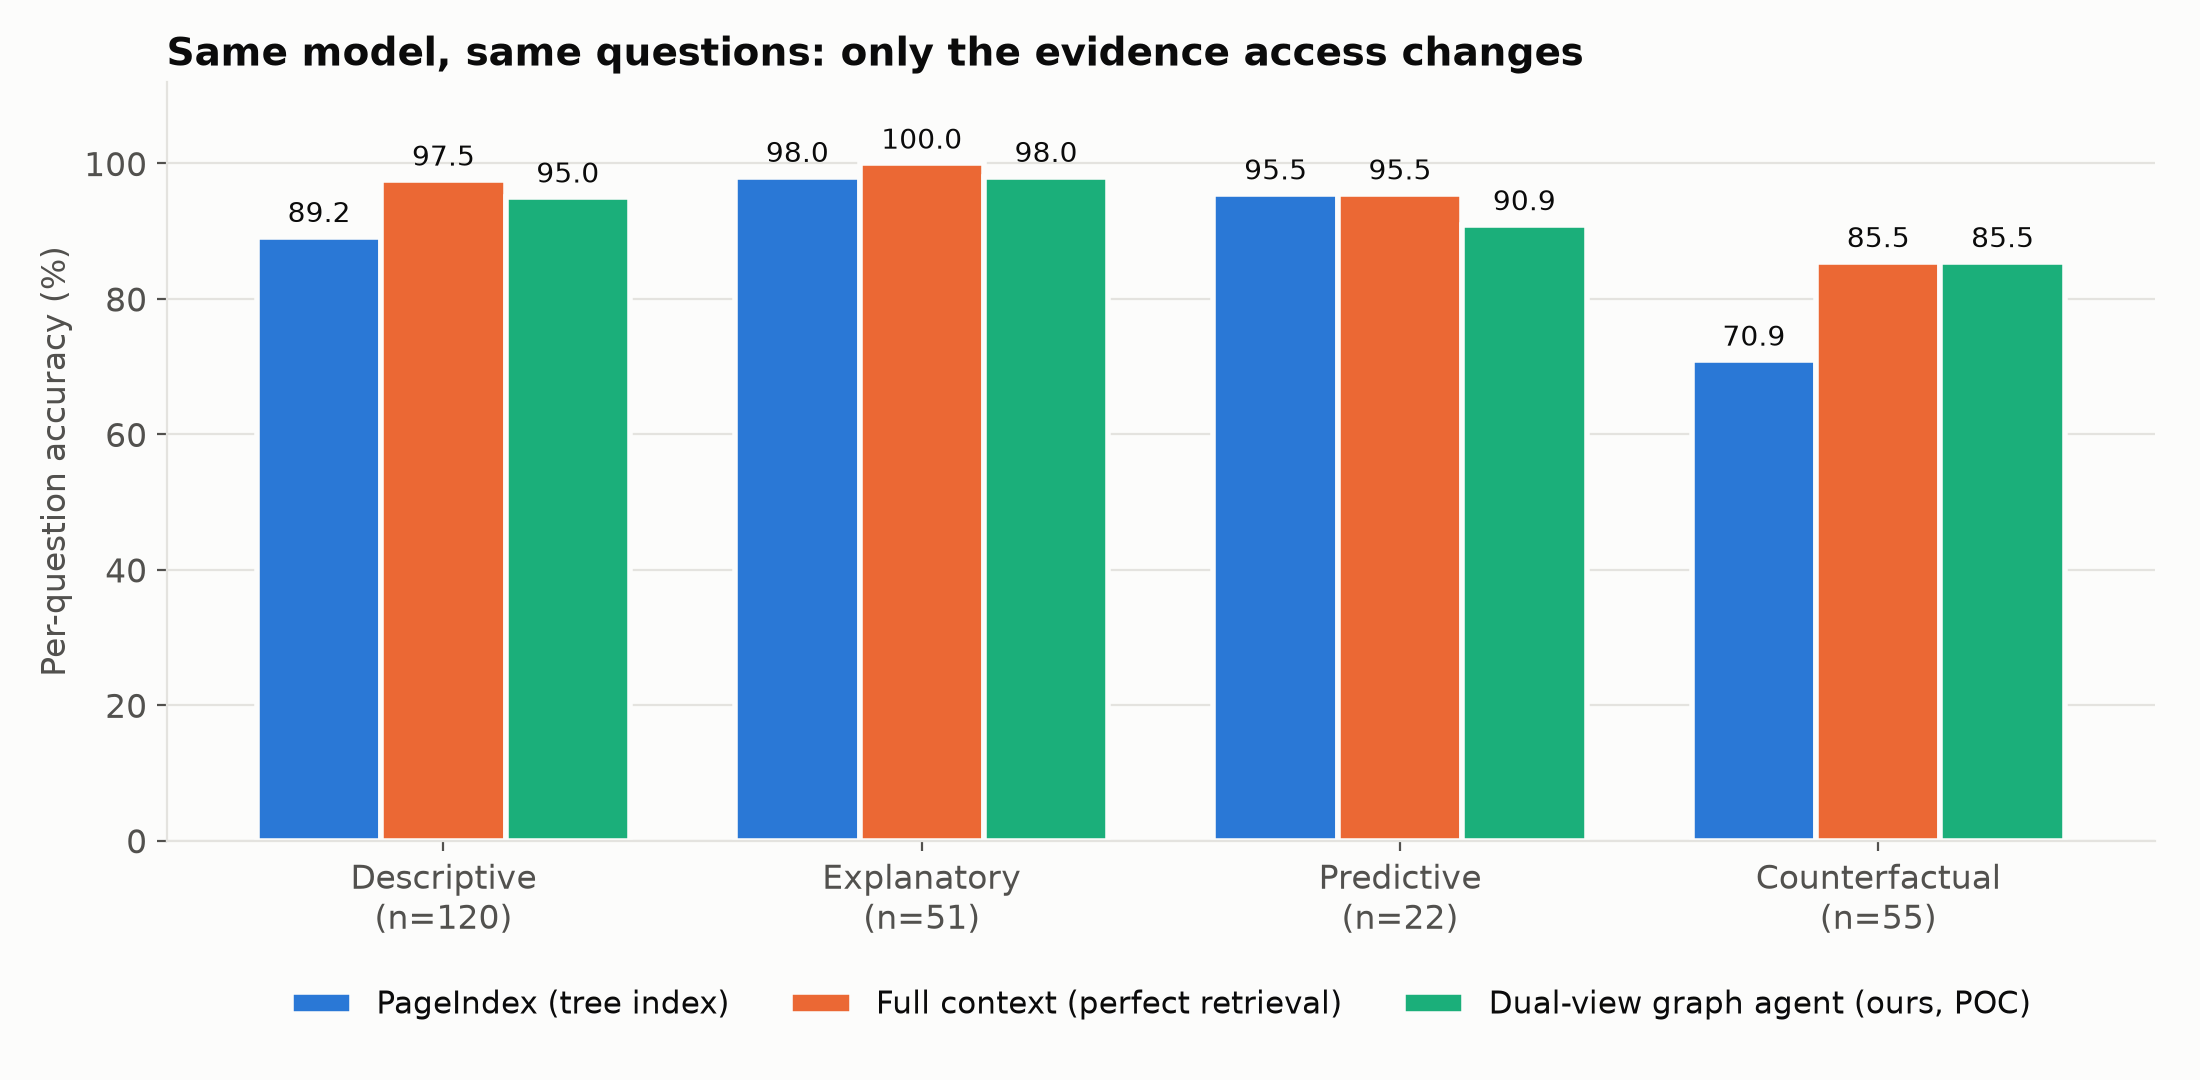
\includegraphics[height=5.75cm]{fig1_accuracy_by_type.png}\par
  \vspace{0.05cm}
  \fnote{Paired on the same questions: full context right and PageIndex wrong on 20 questions; the reverse on 1 (McNemar exact p = 2e-5). Graph agent against PageIndex: 20 to 6 (p = 0.009).}
\end{frame}

% == 5 == Result 2 =============================================================
\begin{frame}{PageIndex is the slowest and most costly system}
  \vspace{0.10cm}
  \centering
  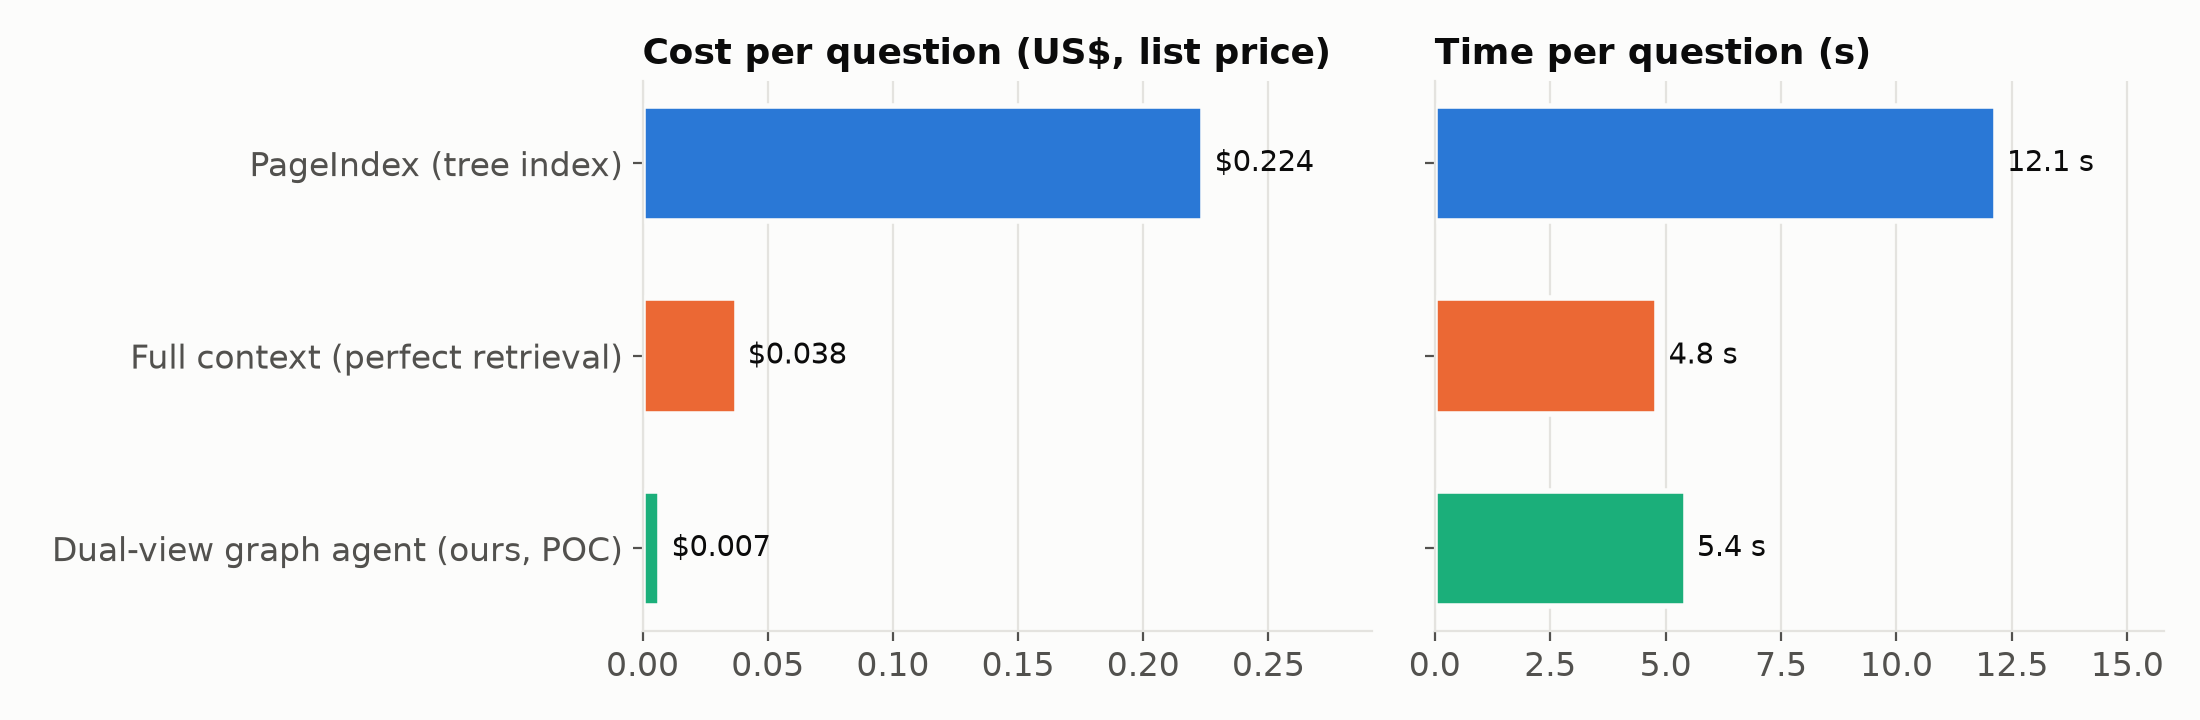
\includegraphics[width=0.86\textwidth]{fig2_cost_time.png}\par
  \vspace{0.10cm}
  \raggedright
  {\fontsize{10}{13}\selectfont
  \begin{itemize}\setlength{\itemsep}{1pt}
    \item 110{,}010 input tokens for each question: 6 times full context, 38 times our agent.
    \item The tree has 361 nodes (about 90{,}000 tokens). The agent reads its parts again in every turn. One run has about 17{,}000 tokens.
  \end{itemize}}
  \vspace{0.05cm}
  \fnote{List price on OpenRouter. Prompt caching made the real bill lower. Total spend for all pilot runs: about \$47.}
\end{frame}

% == 6 == Why 1 ================================================================
\begin{frame}{Why 1: PageIndex reads only part of the right run}
  \vspace{0.15cm}
  \begin{columns}[T,onlytextwidth]
    \begin{column}{0.57\textwidth}
      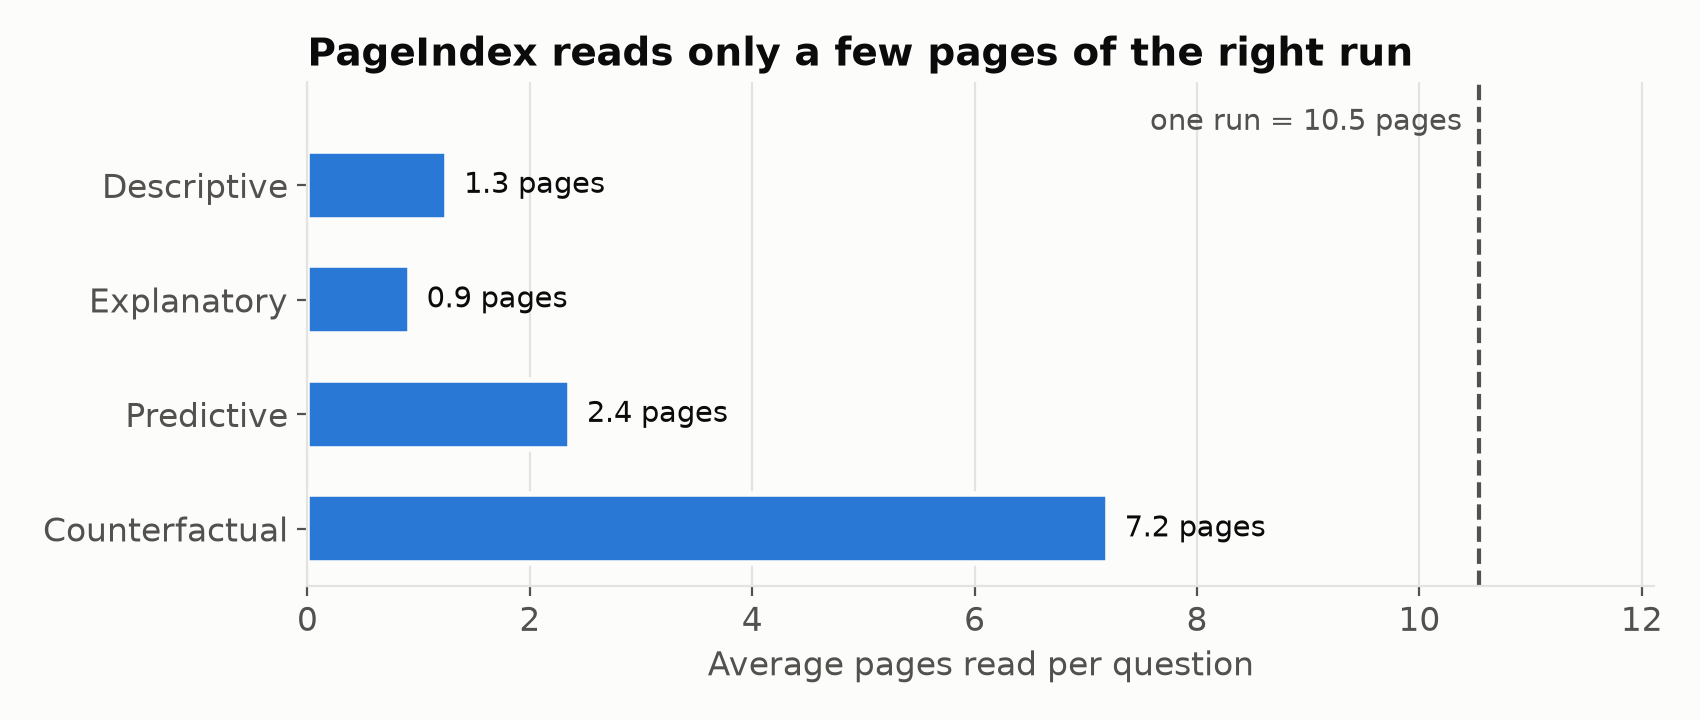
\includegraphics[width=\textwidth]{fig4_pageindex_pages_read.png}
    \end{column}
    \begin{column}{0.39\textwidth}
      \vspace{0.20cm}
      \finding{0}{reads of a wrong run: the table of contents works at chapter level}
      \vspace{0.18cm}
      \finding{4}{errors: the state tables that the question needed were on pages that it did not read}
      \vspace{0.18cm}
      \finding{10\%}{of answers came from the tree summaries alone}
      \vspace{0.25cm}
      \lbl{The tool description tells the agent:}
      {\fontsize{9.5}{12.5}\selectfont\itshape ``Use tight, targeted page ranges, never the whole document at once.''\par}
    \end{column}
  \end{columns}
\end{frame}

% == 7 == Why 2 ================================================================
\begin{frame}{Why 2: the tree is a table of contents}
  \vspace{0.15cm}
  \lbl{The PageIndex tree of our plant log, built from clean headings and bookmarks}
  \vspace{0.06cm}
  {\fontsize{10.5}{13.5}\selectfont
  \begin{itemize}\setlength{\itemsep}{3pt}
    \item \textbf{Merged headings.} One node is titled \code{Run 10307: scene report 10307.1 Overview}.
    \item \textbf{Wrong nesting.} All state tables became children of \code{Event log}. A table header (\code{Frame Event}) became a node.
    \item \textbf{Lossy summaries.} A summary says the frames ``contain object identities only''. The pages hold positions, speeds and states.
    \item \textbf{Page ranges overlap.} A page holds parts of two time windows, so a time question needs more than one node.
    \item \textbf{Evidence in hand, still wrong.} In 11 errors, PageIndex had read the evidence. The same model with only the run's pages got all 11 right.
  \end{itemize}}

\end{frame}

% == 8 == Examples =============================================================
\begin{frame}{Two kinds of failure}
  \vspace{0.20cm}
  \begin{columns}[T,onlytextwidth]
    \begin{column}{0.47\textwidth}
      \lbl{Evidence not read (run 10572)}
      {\color{Ink}\fontsize{11.5}{14.5}\selectfont\bfseries ``How many moving spheres are there?''\par}
      \vspace{0.12cm}
      {\fontsize{10}{13.5}\selectfont
      \begin{itemize}\setlength{\itemsep}{2pt}
        \item Correct answer: 2. The spheres move later in the video.
        \item PageIndex read page 57 only (frames 0 to 15) and answered \textbf{0}.
        \item Full context: 2. Graph agent: 2 (\code{states\_at} at two frames).
      \end{itemize}}
    \end{column}
    \begin{column}{0.47\textwidth}
      \lbl{Evidence read, still wrong (run 10475)}
      {\color{Ink}\fontsize{11.5}{14.5}\selectfont\bfseries ``How many rubber objects enter the scene?''\par}
      \vspace{0.12cm}
      {\fontsize{10}{13.5}\selectfont
      \begin{itemize}\setlength{\itemsep}{2pt}
        \item Correct answer: 2.
        \item PageIndex read page 24. Its event log shows the two rubber objects that enter. It answered \textbf{3}.
        \item Full context: 2. Graph agent: 2 (one \code{event\_log} call).
      \end{itemize}}
    \end{column}
  \end{columns}
\end{frame}

% == 9 == Correction ===========================================================
\begin{frame}{A correction to our hypothesis}
  \vspace{0.25cm}
  \begin{columns}[T,onlytextwidth]
    \begin{column}{0.47\textwidth}
      \lbl{What we expected}
      {\fontsize{10.5}{13.5}\selectfont
      Predictive and counterfactual answers are in no document, so these questions fail.\par}
      \vspace{0.12cm}
      \lbl{What the pilot shows}
      {\fontsize{10.5}{13.5}\selectfont
      With all state tables of the run, the model does the physics: 95.5\% predictive, 85.5\% counterfactual.\par}
      \vspace{0.12cm}
      \lbl{Revised claim}
      {\color{Ink}\fontsize{11}{14}\selectfont\bfseries Tree retrieval does not deliver clean, complete evidence for causal and counterfactual answers.\par}
    \end{column}
    \begin{column}{0.47\textwidth}
      \lbl{Still true: retrieval alone cannot do it}
      {\fontsize{10}{13}\selectfont
      \begin{itemize}\setlength{\itemsep}{2pt}
        \item 100\% of correct predictive answers are events that the video does not show.
        \item 44.8\% of counterfactual questions need such an event.
        \item A causal graph of observed events, with no computation: 29.6\% predictive, 52.1\% counterfactual.
        \item So something must compute the answer: the LLM from raw numbers, or an operator.
      \end{itemize}}
    \end{column}
  \end{columns}
\end{frame}

% == 10 == Operators ===========================================================
\begin{frame}{Our two operators answer without an LLM}
  \vspace{0.10cm}
  \begin{columns}[T,onlytextwidth]
    \begin{column}{0.58\textwidth}
      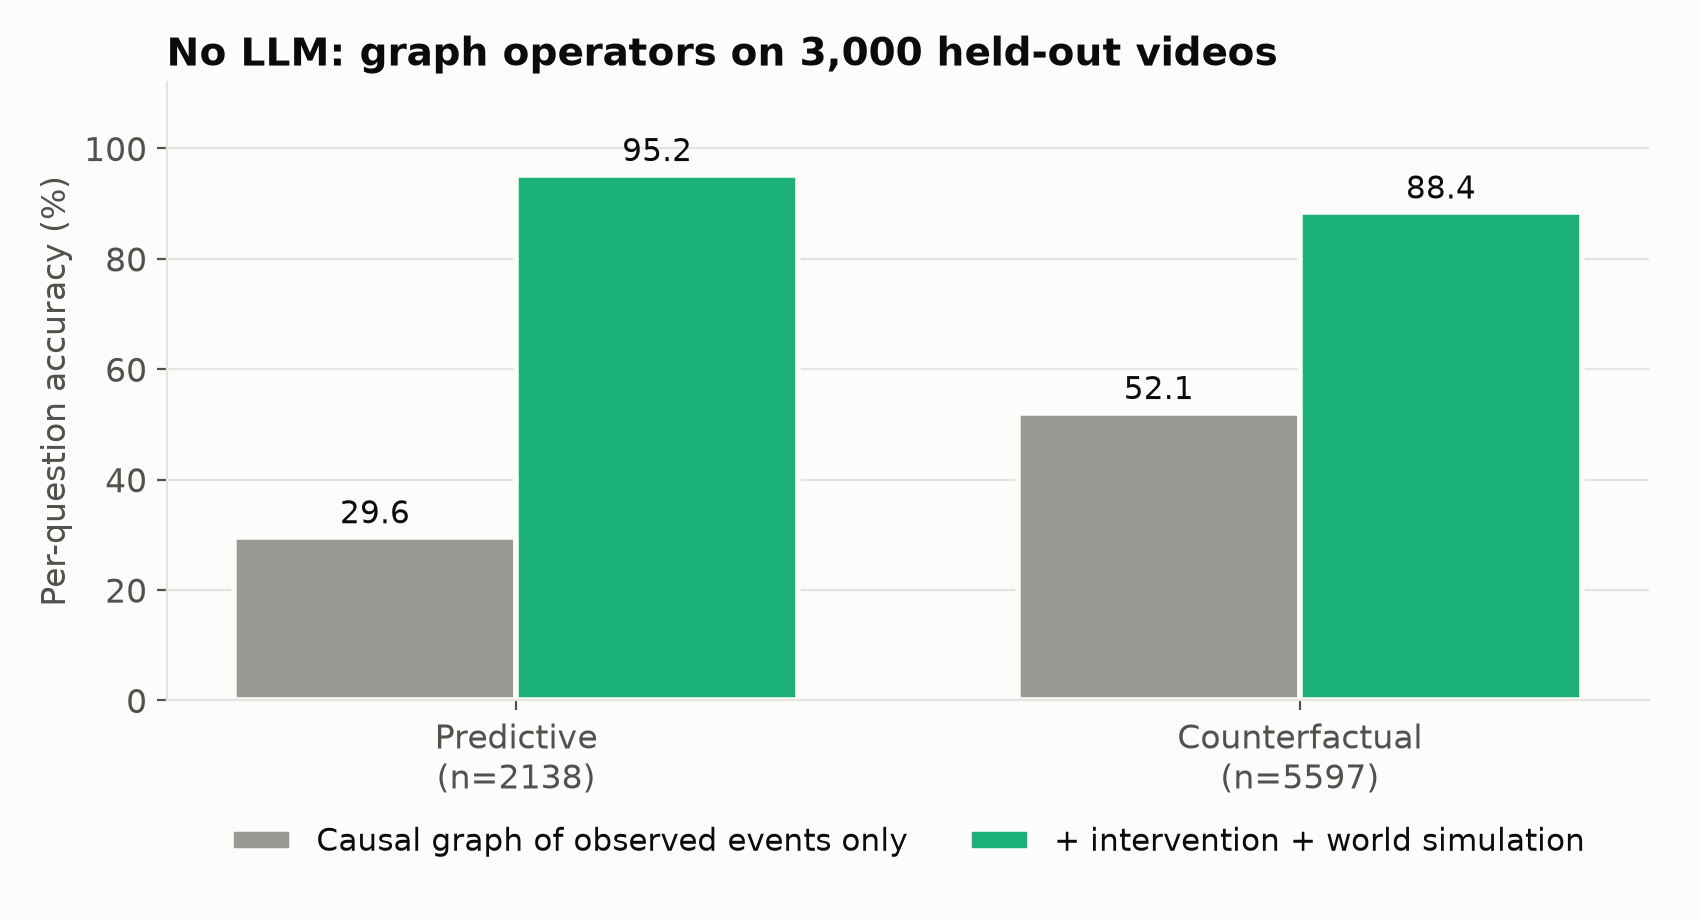
\includegraphics[width=\textwidth]{fig3_operators_heldout.png}
      \vspace{0.10cm}
      \fnote{Best published: 90.7\% counterfactual (CRCG, test split, learned perception). We use ground-truth perception, so this is not a direct comparison.}
    \end{column}
    \begin{column}{0.38\textwidth}
      \vspace{0.15cm}
      {\fontsize{10}{13}\selectfont
      \begin{itemize}\setlength{\itemsep}{3pt}
        \item \textbf{Intervention:} remove object X; find every object whose motion depends on X.
        \item \textbf{World simulation:} straight-line motion with measured friction; detect contacts.
        \item Tuned on videos 10000--11999; scored on held-out videos 12000--14999.
      \end{itemize}}
    \end{column}
  \end{columns}
\end{frame}

% == 11 == Meaning and limits ==================================================
\begin{frame}{What this means, and what we did not test}
  \vspace{0.25cm}
  \begin{columns}[T,onlytextwidth]
    \begin{column}{0.47\textwidth}
      \lbl{Support for the dual-view design}
      {\fontsize{10}{13}\selectfont
      \begin{itemize}\setlength{\itemsep}{2pt}
        \item \textbf{Data graph:} exact state lookups at any frame.
        \item \textbf{Process graph:} the causal past of an event in one call.
        \item \textbf{Operators as tools:} the agent asks for a simulation; it does not read 11 pages of numbers.
        \item Same accuracy as perfect retrieval on counterfactual questions, at 1/6 of its tokens.
      \end{itemize}}
    \end{column}
    \begin{column}{0.47\textwidth}
      \lbl{Limits of this pilot}
      {\fontsize{10}{13}\selectfont
      \begin{itemize}\setlength{\itemsep}{2pt}
        \item Small: 248 questions, only 22 predictive.
        \item Ground-truth perception, not video.
        \item The graph comes from the annotation files, not from the PDF.
        \item No sufficiency check or rollout gating yet.
        \item One model and one corpus size (30 runs).
        \item One tool note changed after one pilot failure.
      \end{itemize}}
    \end{column}
  \end{columns}
\end{frame}

% == 12 == Next steps ==========================================================
\begin{frame}{Next steps and decisions}
  \vspace{0.25cm}
  \begin{columns}[T,onlytextwidth]
    \begin{column}{0.47\textwidth}
      \lbl{Proposed for the next two weeks}
      {\fontsize{10.5}{14}\selectfont
      \begin{enumerate}\setlength{\itemsep}{3pt}
        \item Scale to 500 runs, and a 300-run corpus where full context does not fit.
        \item Build the graph with an LLM from the reports (the offline phase).
        \item Add VLM captions for a perception test on a subset.
        \item Run a lookup benchmark (FinanceBench) to show that we do not lose there.
        \item Start the manufacturing corpus.
      \end{enumerate}}
    \end{column}
    \begin{column}{0.47\textwidth}
      \lbl{Decisions needed today}
      {\fontsize{10.5}{14}\selectfont
      \begin{enumerate}\setlength{\itemsep}{3pt}
        \item Is CLEVRER a diagnostic probe or the main benchmark?
        \item Do operators (intervention, world simulation) become part of the design?
        \item Do we adopt the revised claim (evidence access, not reasoning)?
        \item Which models and which budget?
        \item Which tasks does Ash take?
      \end{enumerate}}
    \end{column}
  \end{columns}
\end{frame}

\end{document}
